\documentclass[12pt, twoside]{article}
\usepackage[letterpaper, margin=1in, headsep=0.5in]{geometry}
\usepackage[english]{babel}
\usepackage[utf8]{inputenc}
\usepackage{amsmath}
\usepackage{amsfonts}
\usepackage{amssymb}
\usepackage{tikz}
\usepackage{yhmath}
\usetikzlibrary{quotes, angles}
\usepackage{graphicx}
\usepackage{enumitem}
\usepackage{multicol}

\newif\ifmeta
\metatrue %print standards and topics tags

\title{Regents Geometry}
\author{Chris Huson}
\date{April 2022}

\usepackage{fancyhdr}
\pagestyle{fancy}
\fancyhf{}
\renewcommand{\headrulewidth}{0pt} % disable the underline of the header
\raggedbottom

\fancyhead[LE]{\thepage}
\fancyhead[RO]{\thepage \\ Name: \hspace{4cm} \,\\}
\fancyhead[LO]{BECA / Dr. Huson / Geometry\\* Unit 10: Trigonometry\\* 6 April 2022}

\begin{document}
\subsubsection*{10.3 Inverse trigonometric functions}
\begin{enumerate}
\item Given right $\triangle ABC$ with $AC=4, BC=5, AB=6.4$, $m\angle C=90^\circ$. Express each trig ratio as a fraction, then as a decimal to the nearest thousandth. (1a is an example)
  \begin{multicols}{2}
    \begin{enumerate}[itemsep=0.2cm]
      \item $\displaystyle \sin A = \frac{5}{6.4} = 0.781$
      \item $\cos A =$
      \item $\tan A =$
    \end{enumerate}
    \begin{center}
      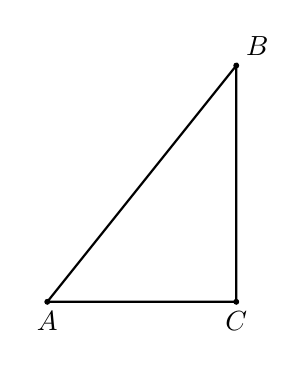
\begin{tikzpicture}[scale=0.6]
        \draw [thick](0,0)--(4,0)--(4,5)--(0,0);
        \draw [fill] (0,0) circle [radius=0.05] node[below]{$A$};
        \draw [fill] (4,0) circle [radius=0.05] node[below]{$C$};
        \draw [fill] (4,5) circle [radius=0.05] node[above right]{$B$};
        %\draw [color=blue] (0,0) ++(0.75,0) arc [start angle=0, end angle=70, radius=0.75];
        %\draw [color=blue] (4,0) ++(-0.22, 0.73) arc [start angle=110, end angle=180, radius=0.75];
        %\draw [thick] (0.8,3.1)--(1.2,2.9); %tick mark
        %\draw [thick] (2.8,2.9)--(3.2,3.1); %tick mark
        %\node [right] at (3.25,2.5){$x+7$};
        %\node [left] at (0.75,2.5){$2x+1$};
      \end{tikzpicture}
    \end{center}
  \end{multicols} \vspace{1cm}

\item Isosceles right triangle $\triangle ABC$ is shown with base $AC=1$ length marked.\vspace{0.25cm}
\begin{multicols}{2}
  \begin{enumerate}[itemsep=0.4cm]
    \item Write down the length of side $BC$.
    \item Find the length of the hypotenuse $AB$.
    \item Write down the angle measures of $\angle A$ and $\angle B$.
    \item Write down $\tan A$.
    \item Write down $\cos A$.\vspace{1cm}
  \end{enumerate}
\begin{flushright}
        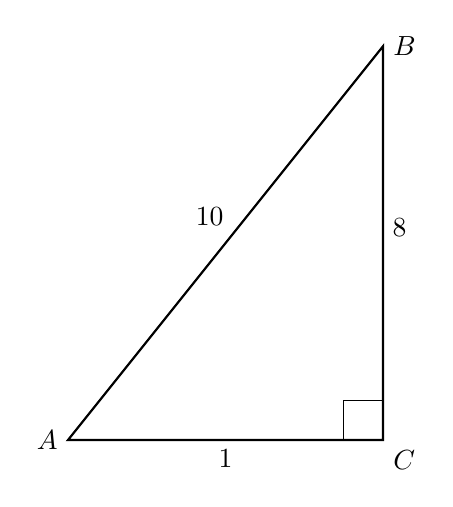
\begin{tikzpicture}[scale=1]
        \draw [thick]
        (0,0)node[left]{$A$}--
        (4,0)node[below right]{$C$}--
        (4,5)node[right]{$B$}--cycle;
        \draw (4,0)++(-0.5,0)--++(0,0.5)--+(0.5,0);
        \node at (2,0)[below]{$1$};
        \node at (4,2.7)[right]{$8$};
        \node at (1.8,2.6)[above]{$10$};
      \end{tikzpicture}
\end{flushright}
\end{multicols} \vspace{1cm}

\item Use the inverse tangent function to find $m\angle A=\theta$ for right $\triangle ABC$ as shown.
  \begin{flushright}
    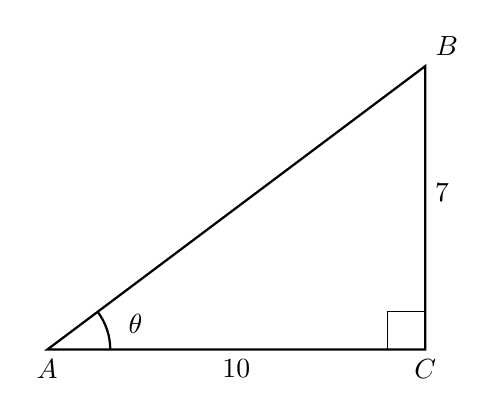
\begin{tikzpicture}[scale=0.8]
      \draw [thick](0,0)node[below]{$A$}--
      (6,0)node[below]{$C$}--
      (6,4.5)node[above right]{$B$}--cycle;
      \draw (6,0)++(-0.6,0)--++(0,0.6)--+(0.6,0);
      \node at (3,0)[below]{$10$};
      \node at (6,2.5)[right]{$7$};
      \draw [thick, -] (1,0) arc [start angle=0, end angle=37, radius=1];
      \node at (1.4,0.1)[above]{$\theta$};
    \end{tikzpicture}
  \end{flushright} \vspace{2cm}

\newpage
\item Triangle $ABC$ is shown with $AB=20.0$, $BC=12.5$, and $m\angle A=90^\circ$. Find $m\angle A$.
  \begin{flushright}
    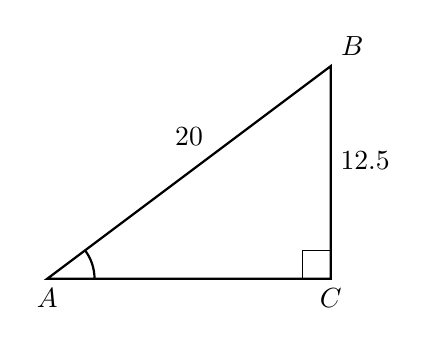
\begin{tikzpicture}[scale=0.6]
      \draw [thick](0,0)node[below]{$A$}--
      (6,0)node[below]{$C$}--
      (6,4.5)node[above right]{$B$}--cycle;
      \draw (6,0)++(-0.6,0)--++(0,0.6)--+(0.6,0);
      \node at (3,3){$20$};
      \node at (6,2.5)[right]{$12.5$};
      \draw [thick, -] (1,0) arc [start angle=0, end angle=37, radius=1];
      %\node at (1.8,0)[above]{$33^\circ$};
    \end{tikzpicture}
  \end{flushright} \vspace{0.5cm}

\item Given right $\triangle JKL$ with $\overline{JK} \perp \overline{KL}$, $JL=12.5$, $JK=10.9$. Find $m\angle J$ in degrees, \emph{rounded to three significant figures}.
  \begin{flushright}
    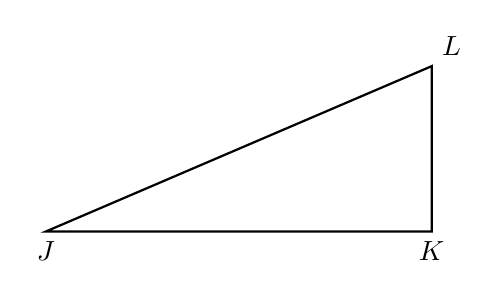
\begin{tikzpicture}[scale=0.7]
      \draw [thick]
      (0,0) node[below]{$J$}--
      (7,0)  node[below]{$K$}--
      (7,3) node[above right]{$L$}--cycle;
    \end{tikzpicture}
  \end{flushright} \vspace{1cm}

\item Given right $\triangle DEF$ with $DE=7, EF=3, DF=7.6$, $m\angle E=90^\circ$. Express each trig ratio as a fraction, then as a decimal \emph{rounded to three significant figures}.
  \begin{center}
    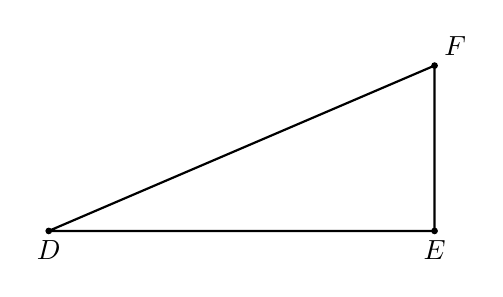
\begin{tikzpicture}[scale=0.7]
      \draw [thick](0,0)--(7,0)--(7,3)--(0,0);
      \draw [fill] (0,0) circle [radius=0.05] node[below]{$D$};
      \draw [fill] (7,0) circle [radius=0.05] node[below]{$E$};
      \draw [fill] (7,3) circle [radius=0.05] node[above right]{$F$};
      %\draw [color=blue] (0,0) ++(0.75,0) arc [start angle=0, end angle=70, radius=0.75];
      %\draw [color=blue] (4,0) ++(-0.22, 0.73) arc [start angle=110, end angle=180, radius=0.75];
      %\draw [thick] (0.8,3.1)--(1.2,2.9); %tick mark
      %\draw [thick] (2.8,2.9)--(3.2,3.1); %tick mark
      %\node [right] at (3.25,2.5){$x+7$};
      %\node [left] at (0.75,2.5){$2x+1$};
    \end{tikzpicture} \vspace{1cm}
  \end{center}
  \begin{multicols}{2}
    \begin{enumerate}
      \item $\sin F = $ \vspace{1cm}
      \item $\cos F =$ \vspace{1cm}
      \item $\tan F =$
      \item $\sin D = $ \vspace{1cm}
      \item $\cos D =$ \vspace{1cm}
      \item $\tan D =$

    \end{enumerate}
  \end{multicols}

\end{enumerate}
\end{document}
  